%%%%%%%%%%%%%%%%%%%%%%%%%%%%%%%%%%%%

\section{5.2. Dados pareados}

%%%%%%%%%%%%%%%%%%%%%%%%%%%%%%%%%%%

\subsection{Observações pareados}

\begin{frame}
\frametitle{Prática}
\justifying
\dq{Foram amostradas aleatoriamente 200 observações em uma pesquisa na High School and Beyond. Os alunos fizeram um teste de leitura e escrita. À primeira vista, parece haver uma diferença entre a pontuação média do teste de leitura e escrita?}

\begin{center}
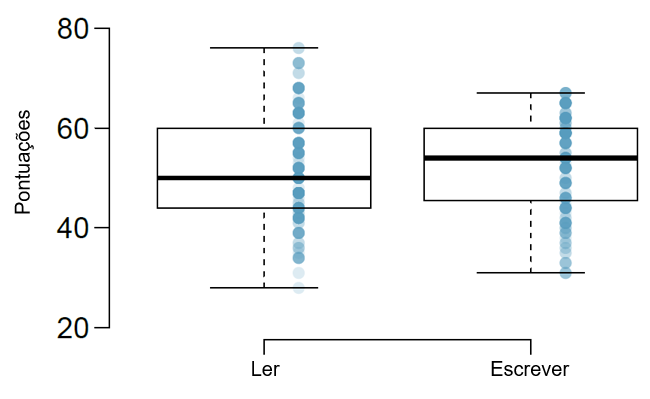
\includegraphics[width=0.5\textwidth]{5-2_paired/hsb2_read_write_box.png}
\end{center}

\end{frame}

%%%%%%%%%%%%%%%%%%%%%%%%%%%%%%%%%%%%

\begin{frame}
\frametitle{Prática}
\justifying
\pq{As notas de leitura e escrita de cada aluno são independentes umas das outras?}

{\small
\begin{center}
\begin{tabular}{rrrr}
  \hline
 & id & leitura & escrita \\ 
  \hline
1 & 70 & 57 & 52 \\ 
  2 & 86 & 44 & 33 \\ 
  3 & 141 & 63 & 44 \\ 
  4 & 172 & 47 & 52 \\ 
  $\vdots$ &   $\vdots$  &   $\vdots$ &   $\vdots$  \\
  200 & 137 & 63 & 65 \\ 
   \hline
\end{tabular}
\end{center}
}

\begin{multicols}{2}
\begin{enumerate}[(a)]
\item Sim
\solnMult{Não}
\end{enumerate}
\end{multicols}

\end{frame}

%%%%%%%%%%%%%%%%%%%%%%%%%%%%%%%%%%%%

\begin{frame}
\frametitle{Analisando dados pareados}
\small
\begin{itemize}
\justifying
\item Quando dois conjuntos de observações têm essa correspondência especial (não independente), diz-se que são \hl{pareados}.

\pause
\justifying
\item Para analisar dados pareados, é frequentemente útil observar a diferença nos resultados de cada par de observações. \\

\centering diferenca = leitura - escrita \\

\pause
\justifying
\item É importante subtrairmos sempre usando uma ordem consistente.

\end{itemize}

\pause
\begin{columns}
\begin{column}{0.5\textwidth}
{\scriptsize
\begin{center}
\begin{tabular}{rrrr >{\columncolor[gray]{.9}}r}
 \hline

 & id & leitura & escrita & diferença \\ 
  \hline
1 & 70 & 57 & 52 & 5 \\ 
  2 & 86 & 44 & 33 & 11 \\ 
  3 & 141 & 63 & 44 & 19 \\ 
  4 & 172 & 47 & 52 & -5 \\ 
  $\vdots$ &   $\vdots$  &   $\vdots$ &   $\vdots$ &   $\vdots$ \\
  200 & 137 & 63 & 65 & -2 \\ 
   \hline
\end{tabular}
\end{center}}
\end{column}
\begin{column}{0.5\textwidth}  %%<--- here
    \begin{center}
     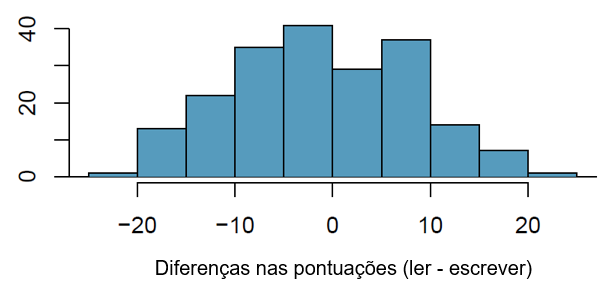
\includegraphics[width=1.15\textwidth]{5-2_paired/hsb2_diff_hist.png}
     \end{center}
\end{column}
\end{columns}

\end{frame}



%%%%%%%%%%%%%%%%%%%%%%%%%%%%%%%%%%%%

\begin{frame}
\frametitle{Estimativa de parâmetro e de ponto}

\begin{itemize}
\justifying
\item \hl{Parâmetro de interesse:} Diferença média entre as pontuações de leitura e escrita de \orange{todos} estudantes do ensino médio.
\[ \mu_{diferenca} \]

$\:$ \\

\pause
\justifying
\item \hl{Estimativa pontual:} Diferença média entre as pontuações de leitura e escrita de estudantes do ensino médio \orange{amostrado}.
\[ \bar{x}_{diferenca} \]

\end{itemize}

\end{frame}

%%%%%%%%%%%%%%%%%%%%%%%%%%%%%%%%%%%%

\subsection{Inferência para dados pareados}

\begin{frame}
\frametitle{Definindo as hipóteses}
\justifying
\dq{Se, de fato, não houve diferença entre as pontuações nos exames de leitura e escrita, como você esperaria que a diferença média fosse?}

\pause

\soln{0}

$\:$ \\

\pause
\justifying
\dq{Quais são as hipóteses para testar se existe uma diferença entre as pontuações médias de leitura e escrita?}

\pause

\begin{itemize}
\justifying
\item[$H_0$:] Não há diferença entre a pontuação média de leitura e escrita.
\[ \mu_{diferenca} = 0 \]
\justifying
\item[$H_A$:] Existe uma diferença entre a pontuação média de leitura e escrita.
\[ \mu_{diferenca} \ne 0 \]
\end{itemize}

\end{frame}

%%%%%%%%%%%%%%%%%%%%%%%%%%%%%%%%%%%%

\begin{frame}
\frametitle{Nada de novo aqui}

\begin{itemize}
\justifying
\item A análise não é diferente do que fizemos antes.
\justifying
\item Temos dados de \orange{uma} amostra: diferenças.
\justifying
\item Estamos testando para ver se a diferença média é diferente de 0.

\end{itemize}

\end{frame}

%%%%%%%%%%%%%%%%%%%%%%%%%%%%%%%%%%%%

\begin{frame}
\frametitle{Verificação de suposições \& condições}
\justifying
\pq{Qual dos seguintes é verdadeiro?}

\begin{enumerate}[(a)]
\justifying
\solnMult{Como os alunos são amostrados aleatoriamente e são menores que 10\% de todos os alunos do ensino médio, podemos supor que a diferença entre os escores de leitura e escrita de um aluno na amostra é independente do outro.}
\justifying
\item A distribuição das diferenças é bimodal, portanto não podemos continuar com o teste de hipóteses.
\justifying
\item Para que as diferenças sejam aleatórias, devemos ter amostras com reposição.
\justifying
\item Como os alunos são amostrados aleatoriamente e são menores que 10\% de todos os alunos, podemos supor que a distribuição amostral da diferença média será quase normal.
\end{enumerate}

\end{frame}

%%%%%%%%%%%%%%%%%%%%%%%%%%%%%%%%%%%

\begin{frame}[shrink]
\frametitle{Calculando a estatística de teste e o valor p}
\justifying
\dq{A diferença média observada entre as duas pontuações é de -0,545 pontos e o desvio padrão da diferença é de 8,887 pontos. Esses dados fornecem evidências convincentes de uma diferença entre as pontuações médias dos dois exames? Usar $\alpha = 0.05$.}

\twocol{0.5}{0.5}
{
\begin{center}
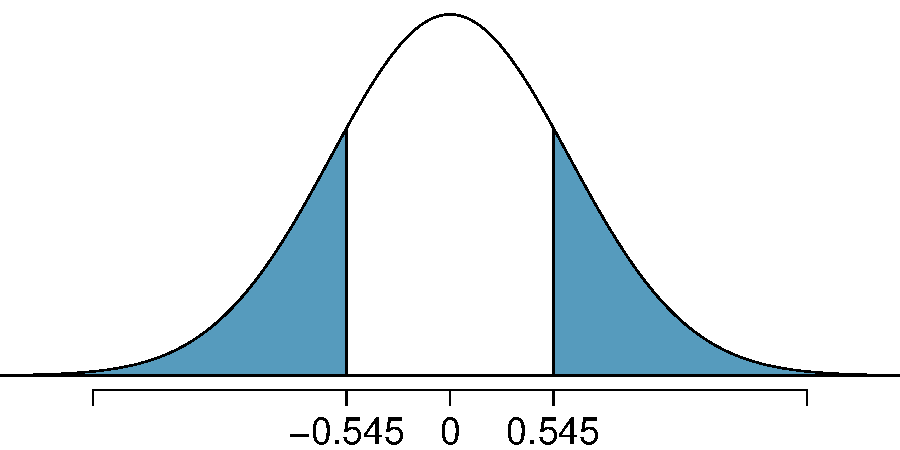
\includegraphics[width=\textwidth]{5-2_paired/hsb2_read_write_pval.pdf}
\end{center}
}
{
\pause
\begin{eqnarray*}
T &=& \frac{-0.545 - 0}{\frac{8.887}{\sqrt{200}}} \\
&=& \frac{-0.545}{0.628} = -0.87 \\
df &=& 200 - 1 = 199 \\
\pause
valor-p &=& 0.1927 \times 2 = 0.3854
\end{eqnarray*}
}
\pause 
$\:$ \\
\justifying
Como o valor de p $> $ 0,05, não é possível rejeitar, os dados \underline {não} fornecem evidências convincentes de uma diferença entre as pontuações médias de leitura e escrita.

\end{frame}

%%%%%%%%%%%%%%%%%%%%%%%%%%%%%%%%%%%

\begin{frame}
\frametitle{Interpretação do valor p}
\justifying
\pq{Qual das seguintes é a interpretação correta do valor p?}

\begin{enumerate}[(a)]
\justifying
\item Probabilidade de que as pontuações médias nos exames de leitura e escrita sejam iguais.
\justifying
\item Probabilidade de que as pontuações médias nos exames de leitura e escrita sejam diferentes.
\justifying
\solnMult{Probabilidade de obter uma amostra aleatória de 200 alunos, onde a diferença média entre as pontuações de leitura e escrita é de pelo menos 0.545 (em qualquer direção), se de fato a diferença média real entre as pontuações é 0.}
\justifying
\item Probabilidade de rejeitar incorretamente a hipótese nula se, de fato, a hipótese nula for verdadeira.
\end{enumerate}

\end{frame}

%%%%%%%%%%%%%%%%%%%%%%%%%%%%%%%%%%%%

\begin{frame}
\frametitle{TH $\leftrightarrow$ IC}
\justifying
\pq{Suponha que fôssemos construir um intervalo de confiança de 95\% para a diferença média entre as pontuações de leitura e escrita. Você esperaria que esse intervalo incluísse 0?}

\begin{enumerate}[(a)]
\justifying
\solnMult{sim}
\justifying
\item não
\justifying
\item não posso dizer a partir da informação dada
\end{enumerate}

\soln{\pause
\begin{eqnarray*} 
-0.545 \pm 1.97 \frac{8.887}{\sqrt{200}} &=& -0.545 \pm 1.97 \times 0.628 \\
&=& -0.545 \pm 1.24 \\
&=& (-1.785, 0.695)
\end{eqnarray*}
}

\end{frame}

%%%%%%%%%%%%%%%%%%%%%%%%%%%%%%%%%%%%

